\section{Development Process}
The exercise was primarily done in the computer lab (room 458 at IT-Vest, NTNU). We chose to use git for version control and GitHub for repository hosting. This allowed us to do minor work off-site, followed by testing at the lab.

The lab had already been set up with multiple workstations running Ubuntu 12.04 LTS with the neccessary software already installed, connected via USB to an EFM32GG-DK3750 development board. A support framework was made available for download that contained some things necessary start programming, such as a vector table and some subroutine headers. This allowed us to get to work on the exercise itself more or less immediately, instead of being caught up in setting things up ourselves.

The exercise description was made available in a compendium also containing instructions about how to write and run the program. Also described was how to use the GNU Debugger to debug. A student assistant was also available a few hours every week to answer questions and provide assistance.

The program itself was developed iteratively with no clearly defined goal, with lots of trial and error along the way. Following the advice in the exercise description, we chose to start by familiarising ourselves with the toolchain and the support files supplied by the subject staff. Subsequently, we implemented a basic version of the program using busy-loop polling, then a version based on interrupts. Finally, we improved energy efficiency by implementing automatic return to a less power intense energy mode after interrupt handling.

\subsection{Devices}
The EFM32GG-DK3750 (figure \ref{img:efm32gg}) connects to a personal computer via USB, shown on the top of the picture. On the device there are multiple GPIO pins. Wires are connected to some of these, and on the other end connected to the gamepad (figure \ref{img:gamepad}). Also integrated on the development board is a energy monitoring unit and a screen that can show a energy monitoring graph.

The gamepad peripheral features 8 LEDs that are toggled via 8 GPIO pins and 8 buttons that control 8 other GPIO pins. The gamepad also has a jumper that can be toggled between two settings. Only if it is "enabled", the amperage powering the LEDs will be registered by the EFM32GG-DK3750 energy monitoring unit.

\begin{figure}[h!]
    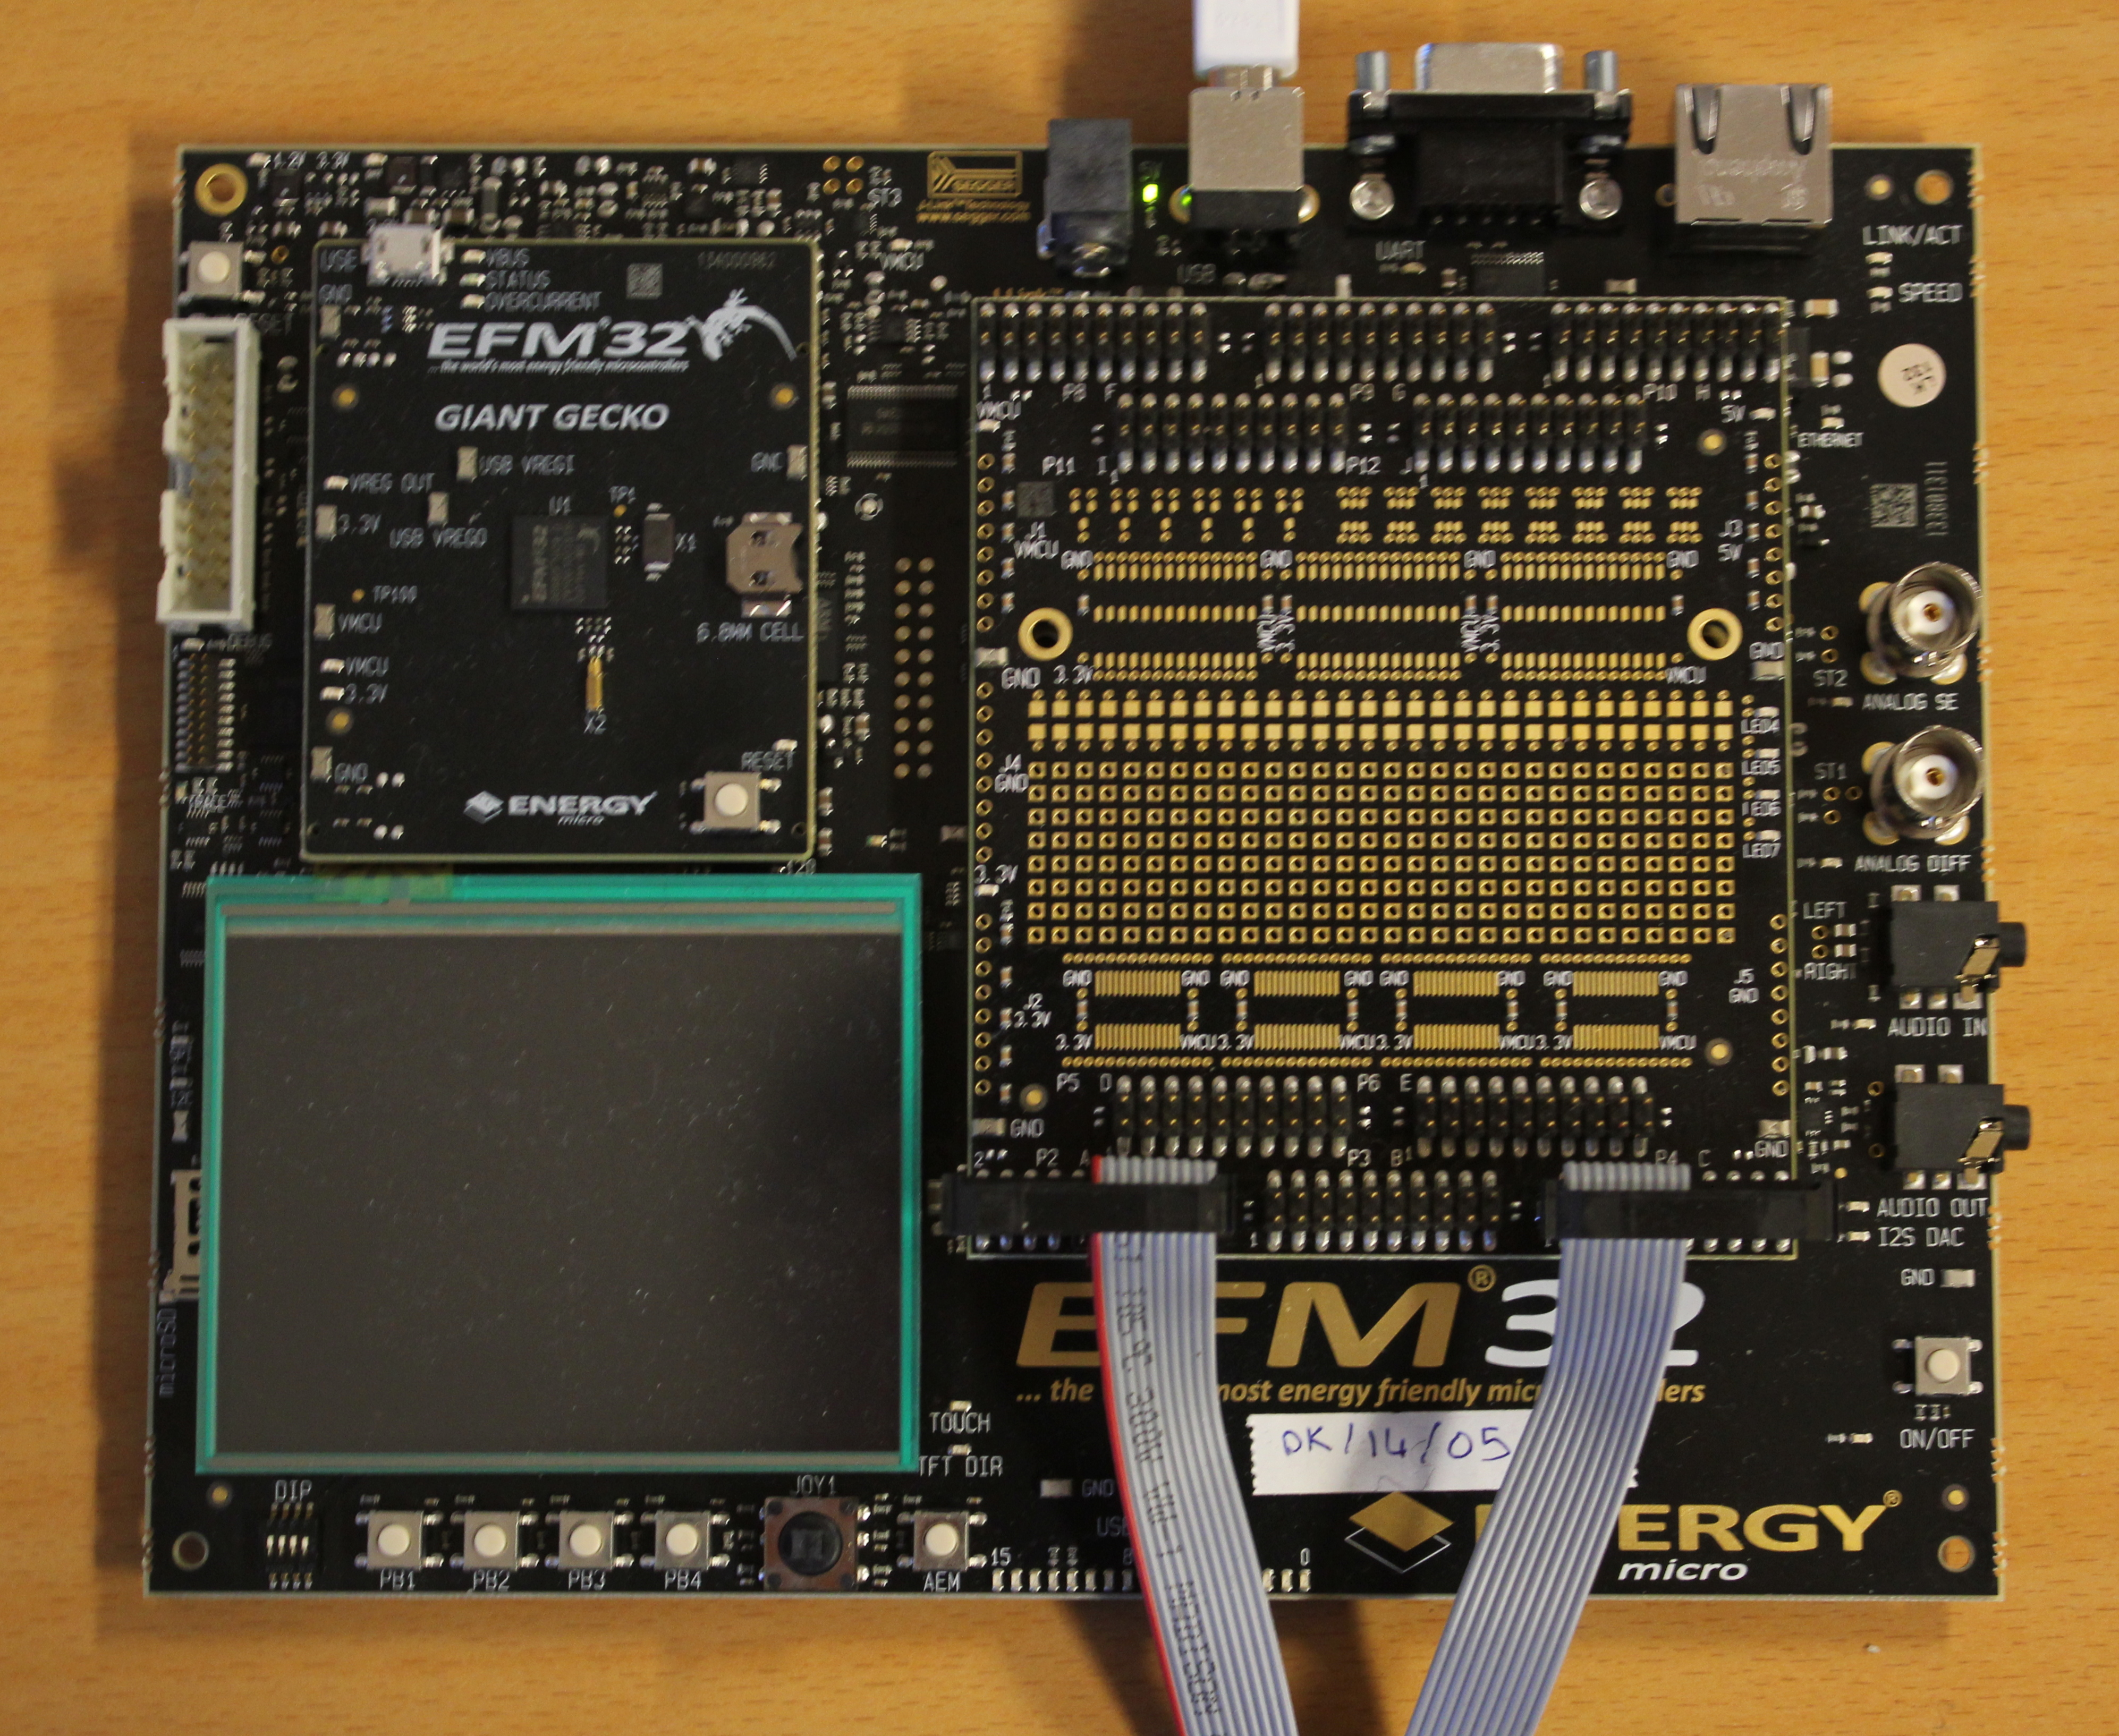
\includegraphics[width=\linewidth]{img/efm32gg.JPG}
    \caption{The EFM32GG-DK3750 \label{img:efm32gg}}
\end{figure}
\begin{figure}[h!]
    \includegraphics[width=\linewidth]{img/gamepad.JPG}
    \caption{The gamepad \label{img:gamepad}}
\end{figure}
